\documentclass{article}

\usepackage{xcolor}
\definecolor{jrouge}{HTML}{CB3C33}
\definecolor{jvert}{HTML}{389826}
\definecolor{jbleu}{HTML}{4063D8}
\definecolor{jviolet}{HTML}{9558B2}
\definecolor{lightred}{HTML}{fcf3f3}
\definecolor{lightgreen}{HTML}{e1f6db}
\definecolor{lightpurple}{HTML}{f4eef7}
\definecolor{lightgrey}{gray}{0.95}

\usepackage{natbib}
%\renewcommand{\citenumfont}[1]{{\tiny#1}}
\renewcommand{\citenumfont}[1]{}
\bibpunct{}{};s;;

\usepackage[top=1.5cm,bottom=1.5cm, left=2.5cm,right=2.5cm]{geometry}
\usepackage[french]{babel}
\usepackage[mathletters]{ucs}
\usepackage[utf8x]{inputenc}
\usepackage[T1]{fontenc}
% Or whatever. Note that the encoding and the font should match. If T1
% does not look nice, try deleting the line with the fontenc.
% Alternative for XeLaTeX:
%\usefonttheme{professionalfonts}
%\usepackage{fontspec}
%\setmonofont{JuliaMono}
%\setdefaultlanguage{french}
%\usepackage{unicode-math}

\usepackage{subcaption}

\usepackage{array}
\usepackage{multirow}
\usepackage{setspace}
\usepackage{soul}
\usepackage{amssymb}
\usepackage{mathrsfs}
\usepackage{bbm}
\usepackage{svg}

\usepackage{tikz}
\usetikzlibrary{scopes, backgrounds, arrows, automata, positioning, patterns, calc, decorations.pathmorphing, decorations.pathreplacing, arrows.meta}

\usepackage{hyperref}
\hypersetup{
	colorlinks=true,
	breaklinks=true,
}
\usepackage{ragged2e}
\usepackage{graphicx}
\usepackage{amsmath}
\usepackage{aeguill}

\usepackage{algorithm}
\usepackage{algpseudocode}
\usepackage{stmaryrd}
\usepackage{siunitx}

\usepackage{forloop}
\newcounter{loop}
\newcounter{numEx}
\newcommand{\exo}[1]{
	\stepcounter{numEx}
	\setcounter{loop}{0}
	\subsection*{Exercice \arabic{numEx} -- #1}
}
\newcommand{\correction}{\textsl{\\Correction de l'exercice \arabic{numEx}\\}}
\newenvironment{corr}{
	\correction	\begin{enumerate}}
	{\end{enumerate}
}

\usepackage{enumitem}
\renewlist{itemize}{itemize}{4}
\setlist[itemize,1]{label={$\bullet$}}
\setlist[itemize,2]{label={$\triangleright$}}
\setlist[itemize,4]{label={$\circ$}}

\newcommand{\llbra}{\left\llbracket}
\newcommand{\rrbra}{\right\rrbracket}
\renewcommand{\brack}[1]{\ensuremath{\llbra#1\rrbra}}
\newcommand{\der}[2]{#1^{\ensuremath{\left(#2\right)}}}
\newcommand{\paren}[1]{\ensuremath{\left(#1\right)}}
\newcommand{\abs}[1]{\ensuremath{\left|#1\right|}}
\newcommand{\interval}[1]{\ensuremath{\left[#1\right]}}
\newcommand{\set}[2]{\ensuremath{\left\{#1\,\middle|\,#2\right\}}}
\newcommand{\cont}[1]{\mathcal{C}^{#1}}
\newcommand{\tends}[2]{\underset{#1\to #2}{\longrightarrow}}
\newcommand{\seq}[3]{\ensuremath{\left(#1_{#2}\right)_{#2\in#3}}}
\newcommand{\matr}[2]{\mathcal{M}_{#1}\paren{#2}}
\newcommand{\matrRect}[3]{\mathcal{M}_{#1,#2}\paren{#3}}
\newcommand{\Id}{\text{Id}}
\newenvironment{disj}[1]{\left\{\begin{array}{#1}} {\end{array}\right.}
\newcommand{\N}{\mathbb{N}}
\newcommand{\R}{\mathbb{R}}
\newcommand{\C}{\mathbb{C}}
\newcommand{\Q}{\mathbb{Q}}
\newcommand{\Z}{\mathbb{Z}}
\newcommand{\K}{\mathbb{K}}
\newcommand{\eps}{\varepsilon}



\title{TD -- Apprentissage de la programmation en Julia}

\author{Lionel~Zoubritzky}

\date{11/2024}

\usepackage{minted}
\usemintedstyle{paraiso-light}
\setminted[julia]{mathescape,linenos,obeytabs,tabsize=4,numbersep=3pt,fontsize=\small,framesep=2mm,autogobble,bgcolor=lightred,escapeinside=££}
\setminted[bash]{mathescape,obeytabs,tabsize=4,numbersep=3pt,fontsize=\small,framesep=2mm,autogobble,bgcolor=lightgrey,escapeinside=££}

\usepackage{lmodern}
%\newcommand{\jl}[1]{\colorbox{lightred}{\small\ttfamily #1}}
\newmintinline[jl]{julia}{}
\newmintinline[jlscript]{julia}{fontsize=\scriptsize}
\newmint[JL]{julia}{}
\newmint[JLa]{julia}{linenos=false}
\newminted{julia}{}
\newenvironment{julia}{\vspace{-0.6em}\VerbatimEnvironment\begin{juliacode}}{\end{juliacode}}
\newminted[jlrepl]{julia}{linenos=false}
\newenvironment{repl}{\vspace{-0.6em}\VerbatimEnvironment\begin{jlrepl}}{\end{jlrepl}}
\newcommand{\q}{\textquotesingle}
\newcommand{\qq}{\textquotedbl}
\newcommand{\jlREPL}{\textcolor{jvert}{\bfseries julia>}}

\DeclareTextFontCommand{\emph}{\bfseries}

\usepackage{xspace}
\newcommand{\expr}{\ensuremath{\left\langle\textit{expr}\right\rangle}\xspace}
\newcommand{\expra}[1]{\ensuremath{\left\langle\textit{expr}_{#1}\right\rangle}\xspace}
\newcommand{\bexpr}{\ensuremath{\left\langle\textit{bexpr}\right\rangle}\xspace}
\newcommand{\bexpra}[1]{\ensuremath{\left\langle\textit{bexpr}_{#1}\right\rangle}\xspace}



\begin{document}
	
\begin{center}
	\Large Apprentissage de la programmation en Julia
	
	TD \no3 : hiérarchie des types et dispatch multiple
	\vspace{2em}
\end{center}

Les questions et exercices annotés du symbole $(*)$ ne sont pas à traiter en priorité.

À chaque question pour laquelle il faut programmer une fonctionnalité, il est implicitement demandé d'inclure un ou plusieurs tests pour s'assurer que l'implémentation est correcte.

Toute fonction non-auxiliaire doit aussi inclure une docstring. Les commentaires sont partout bienvenus.

\exo{Arbres}

Un \emph{arbre} est une structure de données simple représentant une collection d'éléments organisés hiérarchiquement. Sa représentation en mémoire consiste en un ensemble de \emph{nœuds}, ou \emph{branches}, chaque nœud contenant un élément de l'arbre ainsi qu'une liste de sous-nœuds. Une branche qui n'a pas de sous-branche est appelée une \emph{feuille}.

En général, on parle d'arbres sans préciser qu'ils sont implicitement \emph{enraciné}, c'est-à-dire que chaque arbre possède un nœud particulier, appelé \emph{racine}, tel que tout nœud de l'arbre peut être obtenu en suivant des branches connectées entre elles depuis la racine. Une implémentation basique en Julia est :
\begin{repl}
	struct BasicTree  # implicitly a rooted tree
		element
		children::Vector{BasicTree}
	end
\end{repl}

\begin{figure}[bh]
	\centering
	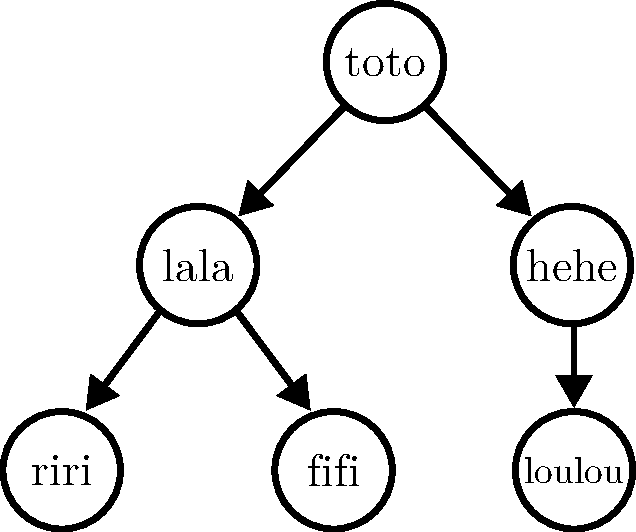
\includegraphics[width=0.5\linewidth]{../figures/tree.pdf}
	\caption{Exemple d'arbre binaire complet. Les nœuds sont les textes entourés. La racine a pour valeur ``toto'' et a deux sous-nœuds, de valeur ``lala'' et ``hehe''. Le sous-arbre ayant pour racine ``hehe'' a deux nœuds : la racine et la feuille ``loulou''.}
\end{figure}

\begin{enumerate}
	\item Définir un type abstrait \jl{AbstractTree{T}} qui représente un arbre dont chaque nœud contient un élément de type \jl{T}.
	
	\item Définir un type \jl{Tree{T}} similaire à \jl{BasicTree}, qui contraint ses éléments à être de type \jl{T}. Comme tous les types d'arbres définis durant ce TD, ce type doit sous-typer \jl{AbstractTree}.
\end{enumerate}

\noindent On définit une interface pour \jl{AbstractTree}. Chaque sous-type doit implémenter :
\begin{itemize}
	\item \jl{root(tree::AbstractTree)} qui renvoie l'élément contenu à sa racine.
	\item \jl{subtrees(tree::AbstractTree)} qui renvoie la liste des sous-arbres extraits depuis chaque sous-nœuds de la racine. Cette liste peut être un \jl{Vector}, un \jl{Tuple}, ou n'importe quel autre type indexable.
\end{itemize}

\begin{enumerate}[resume]
	\item Implémenter cette interface pour \jl{Tree}.
	
	\item Implémenter la fonction \jl{children(tree::AbstractTree)} qui renvoie la liste (\jl{Vector}, \jl{Tuple} ou autre) des éléments contenus dans les sous-nœuds de la racine de \jl{tree}.
	
	Note : cette fonction doit être implémentée de sorte à fonctionner sur n'importe quel sous-type de \jl{AbstractTree}, pas seulement sur un \jl{Tree}.
	
	\item Implémenter le protocole d'itération sur \jl{AbstractTree{T}} de façon à réaliser un parcours en largeur (voir TD précédent). En d'autres termes, une boucle \jl{for x in tree} où \jl{tree isa AbstractTree} doit faire passer \jl{x} par tous les éléments de \jl{tree} en commençant par la racine, puis chacun de ses sous-nœuds dans l'ordre, puis chacun de leurs sous-nœuds en les prenant un par un dans l'ordre, etc., jusqu'à la dernière feuille.
	
	On supposera que la taille d'un \jl{AbstractTree} n'est pas connue à l'avance.
\end{enumerate}

\exo{Arbres binaires}

Un arbre \emph{binaire} est un arbre enraciné donc chaque nœud a au plus deux sous-nœuds.

\begin{enumerate}
	\item Dans quels cas un arbre binaire est-il équivalent à une liste chaînée ?
	
	\item Écrire un type \jl{BinaryTree} permettant d'implémenter un arbre binaire. Le type doit \underline{garantir} que l'arbre est binaire. Comme à l'exercice précédent, il est préférable d'ajouter une variable de type \jl{T} pour préciser le type des éléments de l'arbre.
	\item Écrire un constructeur externe \jl{BinaryTree(l::Vector)} qui crée un arbre binaire à partir d'un vecteur non vide \jl{l}, de sorte que \jl{l[1]} soit la racine et pour tout indice \jl{i} de \jl{l}:
	\begin{itemize}
		\item si \jl{l} a pour taille au moins \jl{2i+1}, alors les sous-nœuds de \jl{l[i]} sont \jl{l[2i]} et \jl{l[2i+1]}.
		\item sinon, si \jl{l} a pour taille exactement \jl{2i}, alors le sous-nœud de \jl{l[i]} est \jl{l[2i]}
		\item sinon, \jl{l[i]} est une feuille.
	\end{itemize}
	
	\item À quelle condition sur \jl{l} un arbre obtenu de la sorte vérifie-t-il la propriété que toutes ses feuilles sont à la même profondeur, c'est-à-dire à la même distance de la racine ? 
	
	Un tel arbre est dit \emph{parfait}. Plus généralement, les arbres obtenus par la méthode précédente sont dits \emph{complets}, c'est-à-dire qu'ils peuvent être obtenus à partir d'arbres parfaits auxquels on aurait enlevé un certain nombre de feuilles, en partant de celles les plus à droite.
	
	\item Expliquer pourquoi, pour toute liste de nombres \jl{l} non vide, \jl{l == collect(BinaryTree(l))}.
\end{enumerate}

On voit ainsi qu'un arbre binaire complet peut avoir différentes représentations en mémoire. La représentation sous forme de vecteur est la plus performante pour des raisons de localité de cache.

\exo{Itération sur les feuilles}

On considère le type suivant :
\begin{repl}
	struct LeafIterator{TreeType}
		tree::TreeType
	
		global leaves  # inner constructor
		leaves(tree::TreeType) where {TreeType<:AbstractTree} = new{TreeType}(tree)
	end
\end{repl}

Implémenter le protocole d'itération sur \jl{LeafIterator} de façon à ce que la boucle \jl{for x in leaves(tree)} où \jl{tree isa AbstractTree} fasse passer \jl{x} par chaque feuille de \jl{tree}.

\exo{Tas}

Un \emph{tas} (\textit{heap}) est un arbre binaire complet \emph{ordonné}, c'est-à-dire que la valeur d'un nœud est inférieure à celle de tous ses sous-nœuds.

\begin{enumerate}
	\item Parmi les arbres représentés ci-après, trouver le seul qui soit un tas.
	
	\item Écrire une fonction \jl{isheap} qui prend un \jl{BinaryTree} et renvoie \jl{true} si c'est un tas, ou \jl{false} sinon.
	
	\item Créer un type \jl{Heap} qui représente le tas sous sa forme de vecteur. En utilisant les questions 3 et 5 de l'exercice précédent, créer un constructeur externe pour \jl{Heap} qui prend un \jl{BinaryTree} en entrée, et, réciproquement un constructeur externe pour \jl{BinaryTree} qui prend un \jl{Heap} en entrée.
	
	\item Créer une méthode \jl{Base.push!(h::Heap{T}, x::T) where {T}} qui ajoute un élément \jl{x} à un tas \jl{h} tout en préservant la propriété du tas. Pour ce faire, l'algorithme consiste à ajouter \jl{x} comme la prochaine feuille, puis à faire remonter \jl{x} dans l'arbre en échangeant \jl{x} avec son parent jusqu'à ce que \jl{x} soit supérieur à son parent. Quelle est sa complexité (dans le pire des cas) ?
	
	\item Créer une méthode \jl{Base.pop!(h::Heap)} qui renvoie la racine du tas et qui la supprime tout en préservant la propriété du tas. Pour ce faire, l'algorithme consiste à déplacer le plus petit des deux sous-nœuds de la racine à sa place, puis à recommencer dans le sous-arbre dont on vient de déplacer la racine, et ce itérativement jusqu'à arriver sur une feuille. Quelle est sa complexité ?
	
	\item Surcharger la fonction \jl{minimum} pour trouver le minimum d'un tas. Quelle est sa complexité ?
	
	\item $(*)$ Proposer un algorithme de tri à base de tas, qui prend en argument une liste de nombres, et qui renvoie la liste triée par ordre croissant.
\end{enumerate}

\exo{Arbre inverse de Syracuse}

On veut construire l'arbre inverse de Syracuse, c'est-à-dire l'arbre des valeurs possiblement prises en suivant une suite de Syracuse à l'envers. Cet arbre est défini de la façon suivante :
\begin{itemize}
	\item La racine vaut \jl{element}, un entier qui correspond au dernier terme de la suite que l'on explore.
	\item Si \jl{element-1} est divisible par trois, alors la racine a deux sous-nœuds, qui sont les arbres inverse de Syracuse ayant pour racine \jl{2*element} et \jl{(element-1)÷3}. Sinon, la racine n'a qu'un seul sous-nœud, qui est l'arbre inverse de Syracuse ayant pour racine \jl{2*element}.
\end{itemize}

\begin{enumerate}
	\item Implémenter l'interface \jl{AbstractTree} sur le type suivant :
	\begin{repl}
		struct InverseSyracuseTree <: AbstractTree{Int}
			element::Int
		end
	\end{repl}
	
	\item Quelle est la taille d'un arbre inverse de Syracuse ? Définir les méthodes appropriée pour que le protocole d'itération défini sur \jl{AbstractTree} reste correct sur \jl{InverseSyracuseTree}.
	
	\item Soit \jl{n} un entier. Comment exprimer le nombre de termes de la suite de Syracuse commençant par \jl{n} et se terminant au premier 1 en fonction du résultat de \jl{findfirst(==(n), InverseSyracuseTree(1))} ?
	
	\item $(*)$ Montrer qu'il existe des couples d'entier $(\jl{n},\jl{m})$ tels que l'appel \jl{findfirst(==(n), InverseSyracuseTree(m))} ne termine pas.
\end{enumerate}

\exo{$(*)$ Algorithme de Dijkstra}

L'algorithme de Dijkstra permet de calculer les plus courts chemins depuis un sommet $s_0$ d'un graphe pondéré dont tous les poids sont positifs. Pour cela, on crée incrémentalement une carte des distances entre le $s_0$ et tous les autres sommets de la façon suivante :
\begin{itemize}
	\item On initialise une carte des distances vide. Cette carte va associer à chaque sommet une distance : on peut l'implémenter avec un dictionnaire initialement vide, ou bien un vecteur intialement rempli de $+\infty$, par exemple.
	\item On initialise un tas en y mettant toutes les paires $(w, i)$ telles que $(s_0, i, w)\in E$. Le tas est ordonné par ordre lexicographique, c'est-à-dire que $(w, i) \le (w', i')$ si et seulement si $w \le w'$ ou [$w = w'$ et $i \le i'$]. La racine du tas contient donc le sommet le plus proche de $s_0$.
	\item À chaque étape, on prend le minimum ($w, i)$ du tas jusqu'à obtenir un $i$ qui n'a pas d'entrée dans la carte des distances. On ajoute alors à cette carte la distance $w$ pour le sommet $i$. Puis, pour chaque arête $(i, j, w')$ partant de $i$ :
	\begin{itemize}
		\item Si $j$ a déjà une distance donnée dans la carte des distances, on ne fait rien.
		\item Sinon, on insère dans le tas $(w + w', j)$.
	\end{itemize}
\end{itemize}
L'algorithme s'arrête lorsque tous les sommets ont une distance associée.

\begin{enumerate}
	\item Montrer que le double invariant suivant est vrai à chaque itération de la boucle principale : ``au début de la $k$-ième étape, la carte contient les $k-1$ sommets les plus proches de $s_0$ et le plus petit poids $w$ associé à un sommet $i$ dans le tas est le plus petit poids d'un chemin entre $s_0$ et $i$ qui ne passe que par des sommets ayant une valeur dans la carte des distances''. En déduire une preuve de l'algorithme.
	
	\item En reprenant le type \jl{WeightedGraph} du TD précédent, implémenter \jl{dijkstra(g::WeightedGraph, s₀)} qui renvoie la carte des distances \jl{map} telle que \jl{map[i]} est la distance minimale entre \jl{s₀} et \jl{i}.
\end{enumerate}
	
\end{document}